Finally, we perform simulations to verify the correctness of the model as well as to simulate an IoT network with varying network configurations. In this section, we present the experimental results of our simulation runs using the model developed in the previous section.

% ===================================== Simulation Parameters ======================================
\subsection{Device Type Comparison}
\label{sub:device_type_comparison}
In all simulations, all devices connected to the network are considered to be using a weak and/or default password, and as such, are vulnerable to a Mirai infection. All infected devices will use a malware binary with a dictionary consisting of 62 commonly used credentials to attack. Unless otherwise mentioned, all devices are one of two types: \AC or \RC, as described in sections~\ref{sub:modeling_always_connected_devices} and~\ref{sub:modeling_reboot_capable_devices}.
\renewcommand{\arraystretch}{1.5}
\begin{table}[h]
    \caption{\label{table:parameters}System Parameters}
    \begin{tabularx}{\linewidth}{| m{0.35\linewidth} c c |}
       \hline 
    	\multicolumn{1}{|c}{Parameter} & Default Value & Other Values Used\\
    	\hline 
    	Number of devices & 100 & 250, 500\\ 
    	Round Trip Time & 100ms & 1s\\ 
    	Simulation time & 1 day & 1 week\\ 
    	Reboot frequency  & 24hr & 1hr, 30min, 10min, 5min\\ 
    	Percentage of time bots propagate malware & 100\% & 50\%, 10\%, 1\%\\ 
    	\hline
    \end{tabularx}
\end{table}
\renewcommand{\arraystretch}{1}
\par
In addition to these constant parameters, Table~\ref{table:parameters} summarizes the adjustable parameters in our model. We perform multiple sensitivity analyses by capturing the model behavior with all parameters set to default and then adjusting one parameter at a time to observe variations in behavior. This allows us to examine how different attributes of the malware, or that of the device network, impact botnet growth. 

\begin{figure}[H]
    \centering
    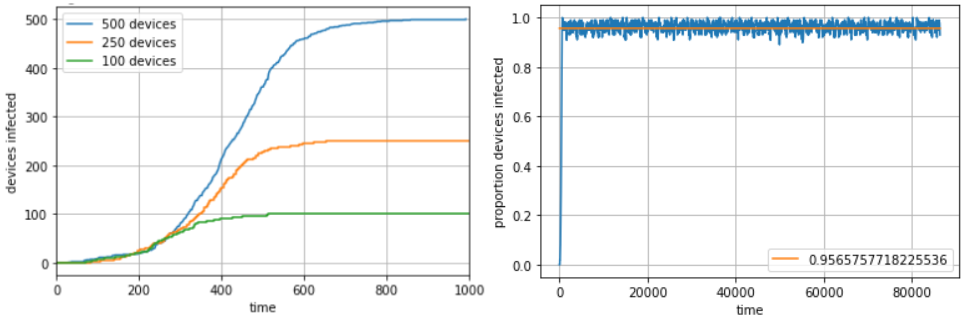
\includegraphics[width=\linewidth]{Figures/Compare_Device_Types.PNG}
    \caption{Botnet Growth for Always-Connected Devices (left) and Reboot-Capable Devices (right)}
    \label{fig:compare_device_types}
\end{figure}
\par

% ===================================== Compare Device Types ======================================
Figure~\ref{fig:compare_device_types} shows the typical behavior of both types of devices. \AC devices maintain their compromised state once infected, producing the expected classical logistic malware growth curve~\cite{stallings_brown_2015}. Once all devices have been infected, no new behavior can occur, so this device type is simulated for a shorter time. \RC devices, on the other hand, can remove their infection through rebooting as this wipes the in-memory malware on the device~\cite{Antonakakis2017_USENIX_Mirai_First_Study}. This produces a graph with a similar logistic growth at the beginning, which eventually settles into a steady-state as devices begin to reboot. This steady-state value is captured for most of the experiments conducted, as this provides an indication of how successful a specific frequency of rebooting is in preventing the botmaster to maintain a certain percentage of devices under their control.
\par
Simulation time is measured relative to the round trip time (RTT) parameter. In Figure~\ref{fig:compare_device_types}, the RTT is one second, so when the \AC devices are all infected within 1000 time units, this is equivalent to 1000 seconds, or 16.67 minutes. The simulation for \RC devices runs for 86400 time units, which for an RTT of one second, is equivalent to one day.

% =====================================  Reboot Frequency ======================================
\subsection{Impact of Rebooting on Percentage of Infected Devices}
\label{sub:rebooting_results}
Table~\ref{table:rebooting} presents the average percentage of infected devices for two networks of 100 devices with different RTTs. Uptime is calculated as the percentage of time a device is connected to the network. For example, a ten minute reboot period means that each device will reboot ten minutes after being connected, and with a fixed reboot length of one minute, has a 90.91\% uptime compared to the total eleven minutes of simulated time. The results indicate that as rebooting is performed more frequently, the average percentage of infected devices decreases, and bots on a slower network are impacted more severely by increased levels of rebooting. 

% old version
%Table~\ref{table:rebooting} presents the average percentage of infected devices for a network of 100 devices. Uptime is calculated as the percentage of time a device is connected to the network based on a one-minute reboot duration. For example, a ten minute reboot period means that each device will reboot ten minutes after being connected, and as the rebooting takes one minute, the uptime is 90\% compared to every ten minutes of simulated time. Botnet sizes are reported identical networks with two different latencies, so we can observe how network speed affects botnet propagation. \todo{3}{What do we see in the table?}

\renewcommand{\arraystretch}{1.5}
\begin{table}[h]
    \caption{\label{table:rebooting}Average percentage of infected devices for different reboot periods}
    \begin{tabularx}{\linewidth}{| c c >{\centering}m{0.263\linewidth} c |}
       \hline 
    	Reboot Period & Uptime & Average percentage  of devices infected (100ms RTT) & \multicolumn{1}{>{\centering}m{0.26\linewidth}|}{Average percentage of devices infected (1s RTT)}\\
    	\hline 
    	24hr & 99.93\% & 99.9\% & 99.0\%\\
    	1hr & 98.36\% & 97.8\% & 95.6\%\\
    	30min & 96.77\% & 96.0\% & 92.1\%\\
    	10min & 90.91\% & 89.6\% & 76.3\%\\
    	5min & 83.33\% & 80.7\% & 46.9\%\\
    	\hline
    \end{tabularx}
    %\vspace{-0.5cm}
\end{table}
\renewcommand{\arraystretch}{1}

% =====================================  Stealthy vs Active ======================================
\subsection{Stealthy vs Active Botnets}
\label{sub:stealthing_results}
%It may be advantageous for a bot to strike a balance between the percentage of time it spends propagating malware, and the percentage of time it stays idle.~\emph{Active} botnets such as Mirai~\cite{kolias2017_Mirai_DDoS} spend more time propagating themselves, so they can grow faster but risk being detected more easily, while \emph{stealthy} botnets will grow slower but are harder to detect. Table~\ref{table:stealthing} reports how different levels of activity, reboot period, and network speed impact the size of a botnet. In extreme cases where a stealthy botnet is operating on a network with a large RTT and frequent rebooting, the botnet is effectively prevented from spreading across the network. More generally, botnets with lower levels of activity achieve lower levels of infection, but a botnet can achieve high levels of stealth before its ability to propagate is affected. As with rebooting, an increase in RTT results in a more dramatic change in botnet size as activity level changes.

It may be advantageous for a bot to strike a balance between the percentage of time it spends propagating malware, and the percentage of time it stays idle.~\emph{Active} botnets such as Mirai~\cite{kolias2017_Mirai_DDoS} spend more time propagating themselves, so they can grow faster but risk being detected more easily, while \emph{stealthy} botnets will grow slower but are harder to detect. Table~\ref{table:stealthing} reports how different levels of activity, reboot period, and network speed impact the size of a botnet. Generally, botnets with lower levels of activity are shown to achieve lower levels of infection, however, bots can be very stealthy without losing much of their propagation capability. As with rebooting, an increase in RTT results in a more dramatic change in the percentage of infected devices as the activity level changes.

%Bots can also be very stealthy without losing much of their propagation capability, especially when devices are rebooted less frequently, as seen from the values reported in Table~\ref{table:stealthing}.

% old version:
%It may be advantageous for a bot to strike a balance between the percentage of time it spends propagating malware and the percentage of time it stays idle. Botnets that spend more time propagating themselves (\emph{active} botnets) can grow faster but risk being detected more easily, whereas botnets which spend more time idle (\emph{stealthy} botnets) will grow slower but are also harder to detect. While the Mirai malware typically is not concerned with hiding its presence~\cite{kolias2017_Mirai_DDoS}, it may be useful to see how different levels of activity affect its growth. Table~\ref{table:stealthing} describes how the activity level for a botnet impact its growth when paired with rebooting and varying network speeds.

\renewcommand{\arraystretch}{1.5}
\begin{table}[h]
    \caption{\label{table:stealthing}Average percentage of infected devices for different levels of botnet stealth}
    \begin{tabularx}{\linewidth}{| >{\centering}m{0.167\linewidth} c c  c |}
       \hline 
    	Percentage of time propagating malware & \multicolumn{1}{>{\centering}m{0.16\linewidth}}{Reboot Period} & \multicolumn{1}{>{\centering}m{0.24\linewidth}}{Average percentage  of devices infected (100ms RTT)} & \multicolumn{1}{>{\centering}m{0.24\linewidth}|}{Average percentage  of devices infected (1s RTT)}\\
    	\hline 
    	100\% & 1hr & 97.8\% & 95.6\% \\ 
    	50\% & 1hr & 97.7\% & 93.2\% \\
    	10\% & 1hr & 95.8\% & 69.6\% \\
    	1\% & 1hr & 71.5\% & 0.0067\% \\
    	100\% & 24hr & 99.9\% & 99.0\% \\
    	50\% & 24hr & 99.7\% & 98.7\% \\
    	10\% & 24hr & 99.4\% & 97.8\% \\
    	1\% & 24hr & 97.4\% & 86.0\% \\
    	\hline
    \end{tabularx}
    \vspace{-0.5cm}
\end{table}
\renewcommand{\arraystretch}{1}